\documentclass[../main.tex]{subfiles}
\begin{document}
\subparagraph{Problem 2}\label{subpar:problem2_fom}

For this second setting we now solve \eqref{eq:heat_fom} for only $N_{\mu}=10$ values of the diffusion parameter but instead of only storing the steady-states we now consider the transient behaviour as well.
Specifically, for each $\mu\in P$, we stack the solutions $\boldsymbol{u}_{h}(t_{n})$, $n=1,\dots,100$, as snapshots in $\boldsymbol{X}$.
In Figure \ref{fig:problem2_fom} we depict such transent behaviour for one diffusion parameter value 

\begin{figure}[H]
    \centering 
    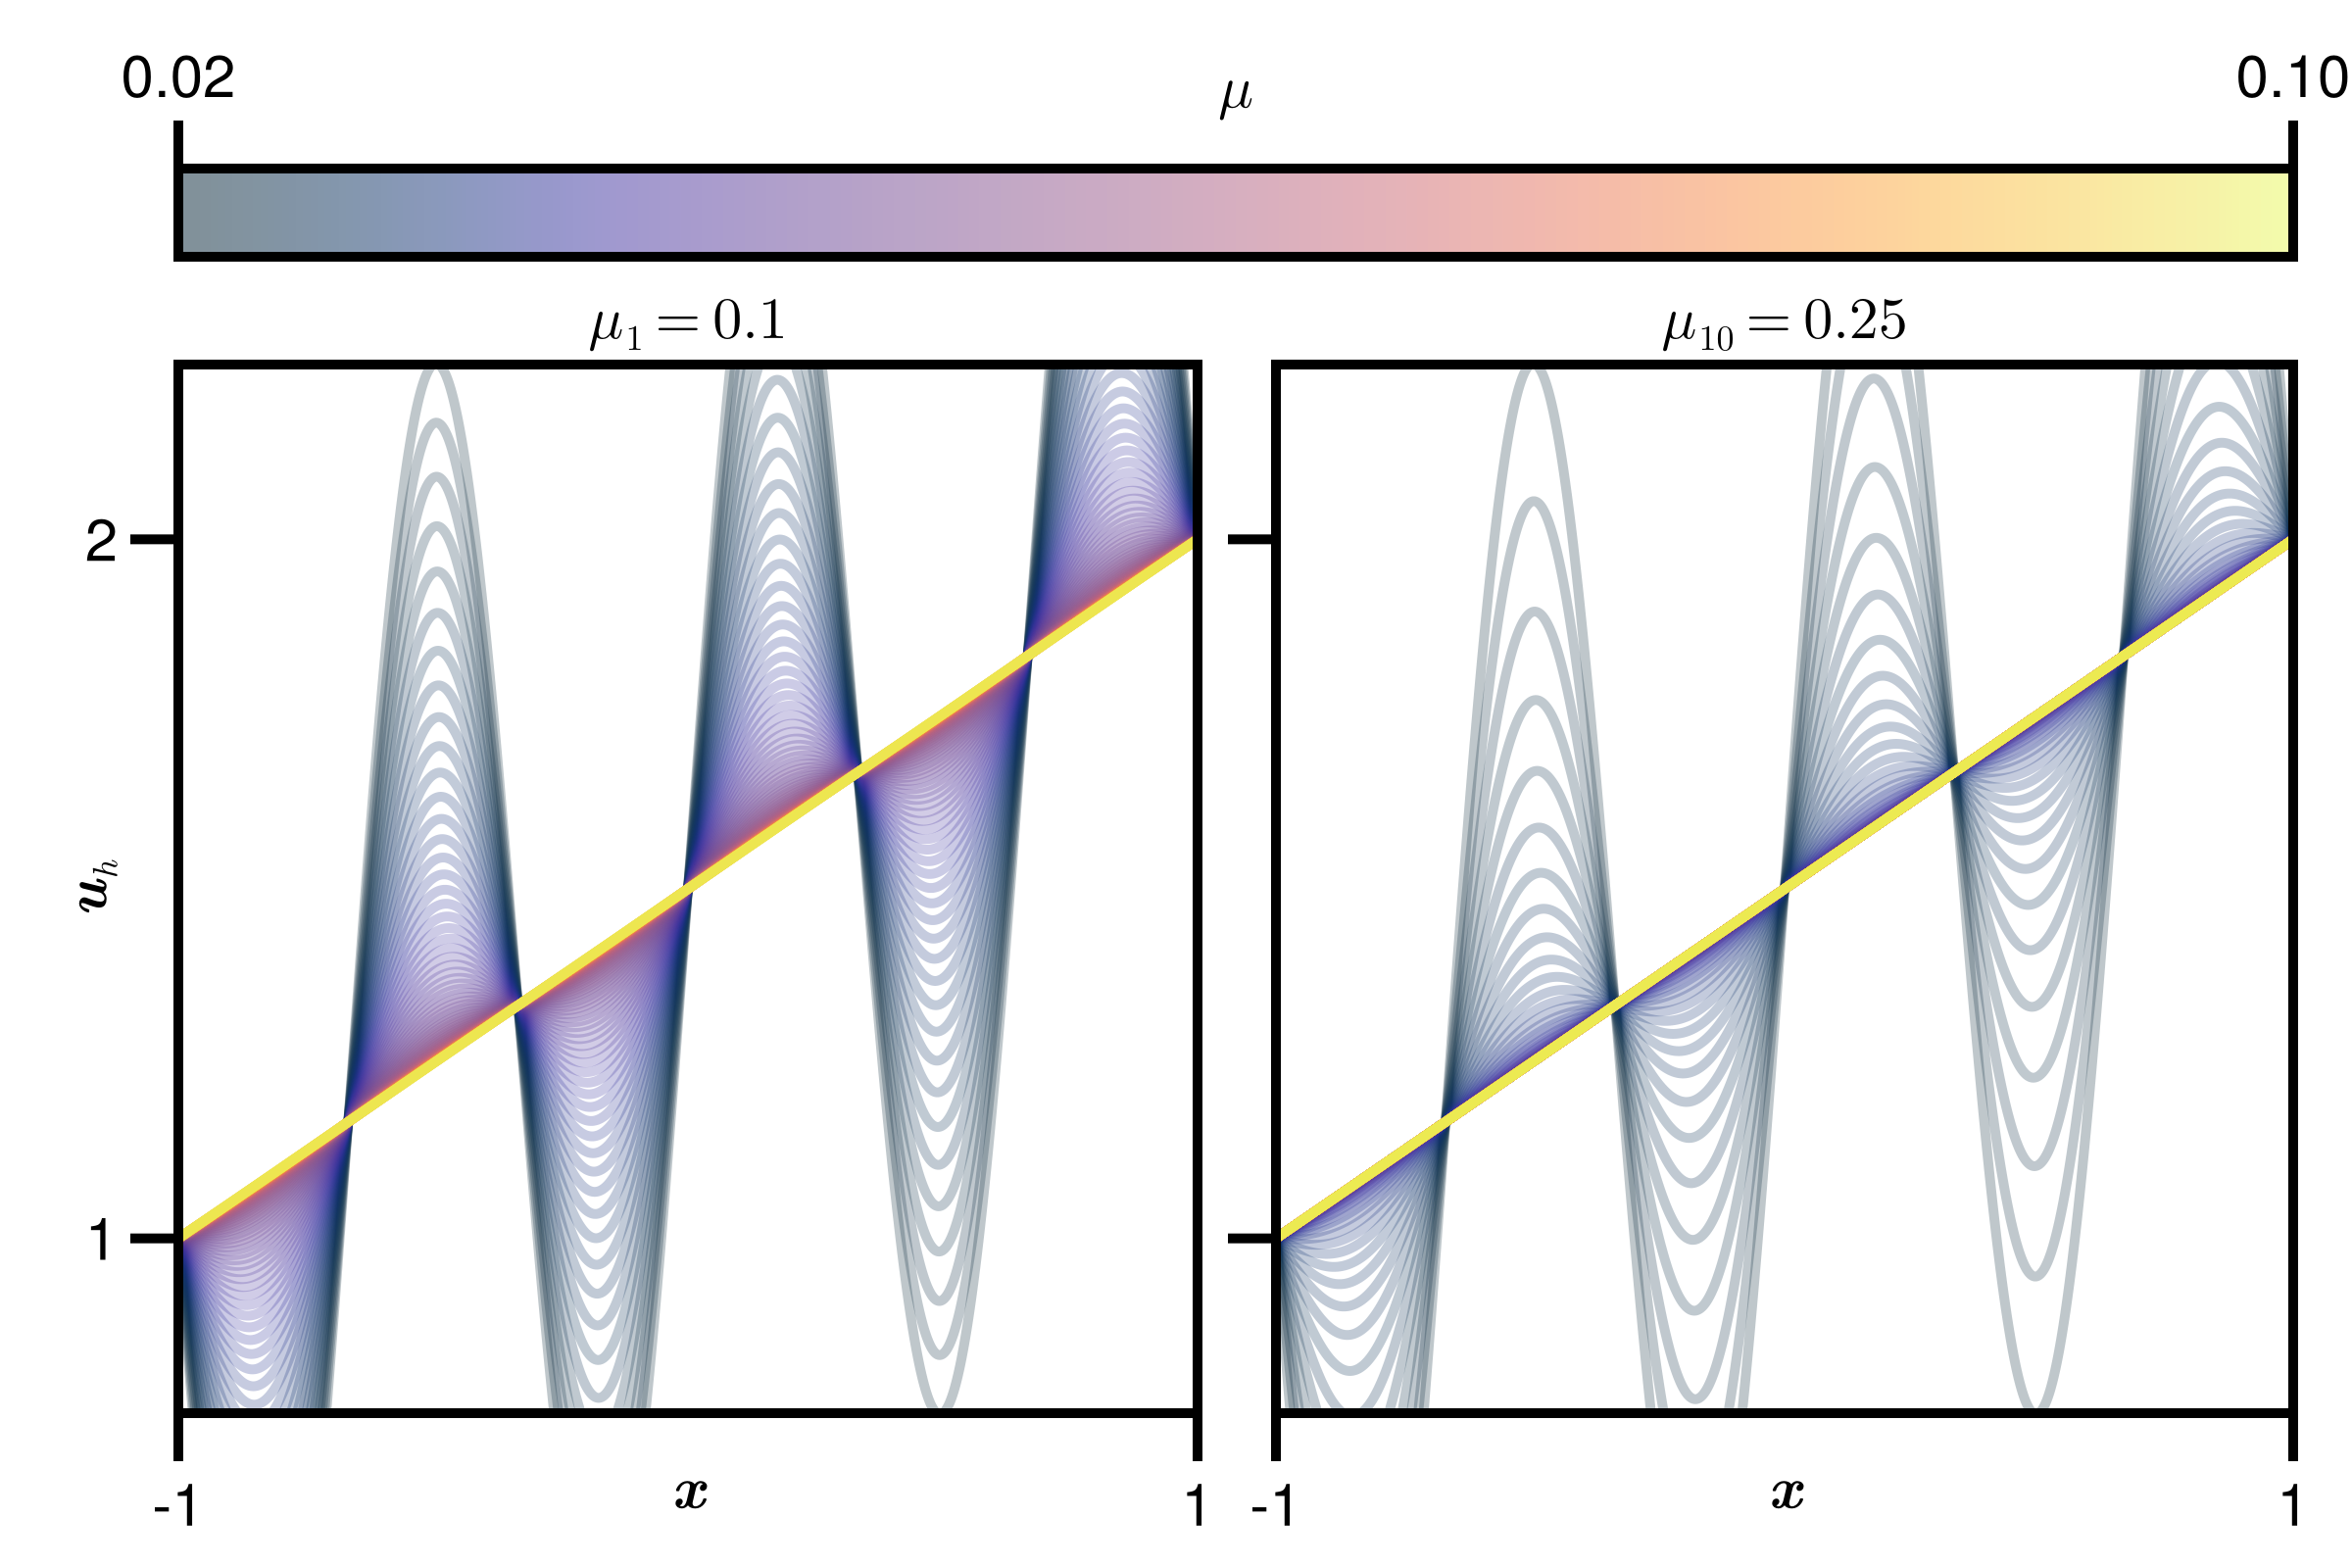
\includegraphics[keepaspectratio, width=0.7\textwidth]{../figures/fig:problem2_fom.png}
    \caption{Time-evolution of two FOM solutions of \eqref{eq:heat_fom} at two different values of the diffusion parameter $\mu\in P$. Notice how at higher values of the diffusion correspond faster relaxation of the patterned IC towards the stable (linear) steady-state as expected.}
    \label{fig:problem2_fom}
\end{figure}

\end{document}
